\documentclass[11pt,reqno]{amsart}
\usepackage[margin=1in]{geometry}
\usepackage{amsmath,amssymb,amsthm,mathtools}
\usepackage{graphicx}
\usepackage[colorlinks=true,linkcolor=blue,citecolor=blue,urlcolor=blue]{hyperref}

\theoremstyle{plain}
\newtheorem{theorem}{Theorem}
\newtheorem{proposition}[theorem]{Proposition}
\newtheorem{lemma}[theorem]{Lemma}
\newtheorem{corollary}[theorem]{Corollary}
\theoremstyle{definition}
\newtheorem{assumption}[theorem]{Assumption}
\theoremstyle{remark}
\newtheorem{remark}[theorem]{Remark}

\newcommand{\dd}{\,\mathrm{d}}
\newcommand{\R}{\mathbb{R}}
\newcommand{\eqd}{\stackrel{d}{=}}
\newcommand{\TW}{\mathrm{TW}}
\newcommand{\Ai}{\mathrm{Ai}}
\newcommand{\Ynode}{Y_{\mathrm{node}}}
\newcommand{\Pearly}{P_{\mathrm{early}}}
\newcommand{\Lam}{\Lambda_0}
\newcommand{\ep}{\varepsilon}
\DeclareMathOperator{\Var}{Var}

\begin{document}

\title[Tracy--Widom statistics of canard escape]{The noisy folded limit cycle:\\
Tracy--Widom statistics of canard escape}
\author{Solomon Williams}
\address{School of Mathematics, University of Edinburgh}
\email{}
\thanks{Draft. Companion technical notes:
\texttt{ShootingCharacterisation\_proof}, \texttt{InstantonPrinciple\_proof},
\texttt{CompositionPropagation\_proof}, \texttt{BlowDown\_proof},
\texttt{ChannelB\_SNIC\_proof}, \texttt{ChannelB\_rigour}.}
\date{\today}

\begin{abstract}
A folded limit cycle is the periodic analogue of a fold singularity in a slow--fast
system: a one-parameter family of limit cycles that loses normal hyperbolicity along a
fold curve. It is the one member of the slow--fast ``fold family'' for which the effect of
noise had not been analysed---Berglund and Gentz treated the fold and the folded node, but
not the folded cycle. We push additive noise through the geometric blow-up of the
folded-cycle fold and identify the law of the noise-induced escape. Linearising the inner
(rescaling-chart) Riccati equation by a Cole--Hopf substitution turns the escape problem
into the first node of a Schr\"odinger equation with a white-noise potential, i.e.\ into
the spectrum of the \emph{stochastic Airy operator} of Ram\'irez--Rider--Vir\'ag. We prove
that the inner exit measure---the law of the slow variable at peel-off---is the
\emph{Tracy--Widom distribution} $\TW_\beta$ with $\beta=4/\eta^2$, $\eta$ the effective
noise; equivalently the canard escape statistics of the folded limit cycle lie in the
Tracy--Widom / KPZ edge universality class. As consequences we obtain the early-escape
probability $1-F_\beta(0)$, a large-deviation rate constant given by a Painlev\'e~II action
$c=5.4439\ldots$, the physical-variable critical-noise law $\sigma_*=2\sqrt\pi\,
\sqrt{\ep_2}\,\sqrt{ac/b}$, and---for the phase (Channel~B) component---a bifurcation-
specific $2/3$ exponent when the cycle is destroyed by a saddle-node on the invariant
circle. All results are confirmed by independent numerical methods, including a
parameter-free comparison with the exact $\TW_\beta$ densities.
\end{abstract}

\maketitle

\section{Introduction}

\subsection{The folded limit cycle}
Slow--fast systems lose normal hyperbolicity at \emph{folds} of their critical manifold,
and the local passage there organises canards, relaxation oscillations and mixed-mode
oscillations. The rigorous tool is geometric desingularisation (``blow-up''), introduced
for the planar fold and canard point by Krupa and Szmolyan \cite{KS}. The same degeneracy
occurs one level up, for a manifold of \emph{limit cycles}: when a one-parameter family of
cycles folds, two cycles (one attracting, one of saddle type) coalesce and annihilate at a
\emph{fold of limit cycles}. Jelbart, Kuehn and Kuntz (JKK) recently carried out the
deterministic blow-up analysis of this folded limit cycle \cite{JKK}, providing a complete
set of charts $K_1$ (entry), $K_2$ (rescaling/inner) and $K_3$ (exit) and a normal form for
the passage.

Real oscillators are noisy, and the effect of noise on slow passage through a fold is the
subject of the Berglund--Gentz sample-path theory \cite{BG}, which treats the planar fold
and---through Berglund, Gentz and Kuehn---the folded node \cite{BGK}. The folded
\emph{limit cycle} is the missing member of this family: the periodicity of the underlying
cycle adds a phase degree of freedom, so the noise acts through two channels, an
\emph{amplitude} channel (escape across the canard) and a \emph{phase} channel (diffusion
of the oscillator phase). This paper analyses both.

\subsection{The result}
Our main finding is that the amplitude channel is, after blow-up, \emph{exactly solvable in
distribution} and connects to random matrix theory. In the rescaling chart $K_2$ the inner
amplitude obeys the canonical noisy Riccati equation
\begin{equation}\label{eq:riccati-intro}
  \dd R=(R^2-Y)\dd T+\eta\,\dd B,\qquad Y=Y_0-T,
\end{equation}
with $\eta$ the effective noise. The deterministic version is the Airy equation (the canard
is $\Ai'/\Ai$, escaping at the first Airy zero); we show the \emph{noisy} version is, via
Cole--Hopf, the eigenvalue equation of the stochastic Airy operator
$H_\beta=-\partial_x^2+x+\tfrac{2}{\sqrt\beta}b'$ of Ram\'irez, Rider and Vir\'ag (RRV)
\cite{RRV}, at the dictionary $\eta=2/\sqrt\beta$. The peel-off level $\Ynode$ (the value of
the slow variable where the trajectory leaves the canard) is the ground-state eigenvalue,
and hence Tracy--Widom distributed.

\begin{theorem}[informal; see Theorems~\ref{thm:shoot}, \ref{thm:escape},
\ref{thm:blowdown}]\label{thm:intro}
The inner exit measure of the noisy folded limit cycle is $\TW_\beta$ with $\beta=4/\eta^2$.
Consequently the early-escape probability is $\Pearly=1-F_\beta(0)$ (with $F_\beta$ the
Tracy--Widom CDF), the early-escape rate is $\exp(-c/\eta^2)$ with $c=5.4439\ldots$ a
Painlev\'e~II action, and in physical variables the critical noise is
$\sigma_*=2\sqrt\pi\,\sqrt{\ep_2}\,\sqrt{ac/b}$.
\end{theorem}

To our knowledge this is the first time a fold/canard escape law has been identified with
the stochastic Airy spectrum. The identification is robust: a Monte-Carlo histogram of
$\Ynode$ overlays the exact $\TW_1,\TW_2$ densities (computed from Painlev\'e~II) with no
fitting (Figure~\ref{fig:twpdf}), and an entirely independent random-matrix computation of
the eigenvalue reproduces the same law (Figure~\ref{fig:dual}).

\subsection{Methods and structure}
The proof proceeds inside the blow-up charts and is assembled back to the physical system.
Section~\ref{sec:setup} recalls the normal form and blow-up. Section~\ref{sec:results}
states the main theorems. Section~\ref{sec:amplitude} develops the amplitude channel: the
exact Cole--Hopf identity (Lemma~\ref{lem:colehopf}), the reduction to the stochastic Airy
operator, and the \emph{shooting characterisation} (Theorem~\ref{thm:shoot}) that the swept
first-node law equals the operator's ground state, proved through a monotone spectral
function that converts a random level into a deterministic one.
Section~\ref{sec:escape} extracts the escape probability and the rate constant $c$ as a
Freidlin--Wentzell / Schilder large deviation. Section~\ref{sec:blowdown} carries the
$\theta$-uniform chart estimates through the composition $\Pi_1\circ\cdots\circ\Pi_3$ and
blows them down to the physical $(\sigma,\ep_2)$ variables.
Section~\ref{sec:phase} treats the phase channel and its bifurcation-specific $2/3$
exponent. Section~\ref{sec:numerics} collects the numerical validation, and
Section~\ref{sec:discussion} discusses universality and applications.

Throughout, results that rest on the established RRV \cite{RRV} and Berglund--Gentz
\cite{BG} frameworks are flagged as such; these are used as cited black boxes, exactly as
the deterministic backbone uses JKK \cite{JKK}.

\section{Setup: normal form and blow-up}\label{sec:setup}

\subsection{The normal form}
Near the folded-cycle fold the JKK reduction \cite{JKK} gives, for the amplitude $r$, slow
variable $y$ and phase $\theta$,
\begin{equation}\label{eq:phys}
  \dd r=\bigl(b(\theta)r^2-a(\theta)y\bigr)\dd t+\sigma\,\dd W_t,\qquad
  \dd y=-\ep_2\,c(\theta)\,\dd t,\qquad \dot\theta=\ep_1,
\end{equation}
with $a,b,c\colon S^1\to\R$ smooth, $1$-periodic and strictly positive, and
$0<\ep_2\ll\ep_1\ll1$, $\ep_1=\ep^\alpha$, $\ep_2=\ep^3$. The deterministic part is JKK's;
the additive noise $\sigma\dd W$ is the new ingredient. The exponent $\alpha$ controls the
phase: $\alpha=2$ freezes $\theta$ over the passage, $\alpha=1$ makes it fast.

\subsection{The fold blow-up}
The Krupa--Szmolyan fold blow-up \cite{KS} is the quasi-homogeneous map with weights
$(1,2,3)$ on $(r,y,\ep_2)$, covered by the charts $K_1,K_2,K_3$. The central rescaling
chart $K_2$ ($\rho=\ep_2^{1/3}$) is
\begin{equation}\label{eq:K2}
  r=\ep_2^{1/3}R,\qquad y=\ep_2^{2/3}Y,\qquad T=\ep_2^{1/3}t,
\end{equation}
under which \eqref{eq:phys} becomes (after the linear rescaling absorbing $a,b,c$) the
canonical inner Riccati \eqref{eq:riccati-intro}, with
\begin{equation}\label{eq:eta}
  \eta=\sigma/\sqrt{\ep_2}
\end{equation}
the effective noise. Equation~\eqref{eq:eta} is an exact change of variables (an It\^o
calculation on a diffeomorphism; Proposition~\ref{prop:noise}). The deterministic inner
solution is the canard $R=\Ai'(Y)/\Ai(Y)$, which escapes to $+\infty$ at the first Airy zero
$Y=a_1\approx-2.3381$.

\subsection{The two channels}
Linearising \eqref{eq:phys} about the canard splits the noise response. The amplitude
channel is \eqref{eq:riccati-intro}; the integrated Kramers hazard for crossing the
separatrix is, in closed form,
\begin{equation}\label{eq:hazard}
  H(\eta)=\frac1\pi\int_0^\infty\!\sqrt Y\,e^{-8Y^{3/2}/3\eta^2}\dd Y=\frac{\eta^2}{4\pi},
\end{equation}
which gives escape at $\eta_*=2\sqrt\pi$ and underlies the critical-noise law. The phase
channel is the noise-driven evolution of $\theta$, regular when the cycle dies at finite
period (fold of cycles) but singular when it dies at infinite period (saddle-node on the
invariant circle); see Section~\ref{sec:phase}.

\section{Main results}\label{sec:results}

We write $\Ynode$ for the peel-off level (the value of $Y$ at the first node of the
Cole--Hopf solution; Section~\ref{sec:amplitude}), $\Lam(\beta)$ for the ground-state
eigenvalue of the stochastic Airy operator $H_\beta$, and $\TW_\beta$, $F_\beta$ for the
Tracy--Widom law and CDF.

\begin{theorem}[reduction and shooting characterisation]\label{thm:shoot}
For the inner Riccati \eqref{eq:riccati-intro} with $\eta=2/\sqrt\beta$, the peel-off level
satisfies
\[
  \Ynode\eqd-\Lam(\beta)\eqd\TW_\beta .
\]
\end{theorem}

\begin{theorem}[escape probability and rate]\label{thm:escape}
The early-escape probability (peel-off before the fold, $\Ynode>0$) is
$\Pearly(\eta)=1-F_\beta(0)$, $\beta=4/\eta^2$. As $\eta\to0$,
\[
  \Pearly(\eta)=\exp\!\bigl(-c/\eta^2\,(1+o(1))\bigr),\qquad
  c=\int_0^\infty g'^2=5.4439\ldots,
\]
where $g$ solves the nonlinear-Airy ground state $-g''+xg=g^3$; $c$ is the action of an
$\alpha=0$ Painlev\'e~II transcendent.
\end{theorem}

\begin{theorem}[physical-variable law]\label{thm:blowdown}
For the original system \eqref{eq:phys}, the peel-off level is $y_{\rm peel}=
\ep_2^{2/3}\Ynode$ with $\Ynode\eqd\TW_{4\ep_2/\sigma^2}$, and escape becomes likely at the
critical noise
\[
  \sigma_*=2\sqrt\pi\,\sqrt{\ep_2}\;G,\qquad
  G=\sqrt{a(\theta_*)c(\theta_*)/b(\theta_*)}\ (\alpha=2),\quad
  \sqrt{\langle a\rangle\langle c\rangle/\langle b\rangle}\ (\alpha=1),
\]
uniformly in $\theta$. All three laws depend on $(\sigma,\ep_2)$ only through
$\eta=\sigma/\sqrt{\ep_2}$ at leading order, in the single-escape regime $\eta\lesssim1$
(Remark~\ref{rem:regime}).
\end{theorem}

\begin{remark}[regime of validity and the recrossing crossover]\label{rem:regime}
Theorems~\ref{thm:shoot}--\ref{thm:blowdown} describe a \emph{single committed} peel-off and
hold as $\eta\to0$. Simulation of the full bistable normal form (subcritical Hopf $+$ fold of
cycles, retaining the coexisting rest state) separates two effects (Fig.~\ref{fig:breakdown}).
The peel-off \emph{distribution} is robust far beyond the asymptotic regime: its standardised
law stays Tracy--Widom to Monte-Carlo accuracy up to $\eta\approx2$. What fails is the
\emph{identification} of the peel-off with one escape---for $\eta=O(1)$ the trajectory can
recross to the cycle. The recrossing probability is below $1\%$ for $\eta\lesssim1.2$, reaches
$5\%$ near $\eta\approx1.5$ and exceeds $30\%$ by $\eta\approx2$. Recrossing is a Kramers
excursion over the unstable cycle ($U(r)=-\tfrac12\mu r^2-\tfrac14 r^4+\tfrac16 r^6$), so the
expected number of returns is $N_{\rm ret}=(C/\ep_2)\,e^{-\Delta U_*/\sigma^2}$. We verify this
directly: $\log(\ep_2 N_{\rm ret})$ is linear in $1/\sigma^2$ with three ramp rates
($\ep_2\in\{1,2,4\}\times10^{-3}$) collapsing onto a single line (Fig.~\ref{fig:boundary};
$R^2=0.93$), with effective barrier $\Delta U_*\approx0.022$ of the order of the normal-form
cycle-to-rest barrier $U(r_u)-U(r_s)$, whereas $P_{\rm recross}$ does \emph{not} collapse in
$\eta$. The breakdown is therefore an Arrhenius (static-Kramers) boundary
$\sigma^2\sim\Delta U_*/\log(1/\ep_2)$ in the $(\sigma,\ep_2)$ plane---weakly (logarithmically)
rate-dependent rather than a fixed $\eta$---i.e.\ the classical critical noise
$\sigma_{\rm crit}$ re-emerging as the ceiling of the Tracy--Widom regime, whose own scale is
the dynamic $\sigma_*\sim\sqrt{\ep_2}$ lying far below it. For $\eta\gtrsim\eta_*\approx1.2$
(at $\ep_2=4\times10^{-3}$) the governing observable crosses from the Tracy--Widom
first-passage law to this two-way transition rate; the clean Tracy--Widom regime is
$\eta\lesssim1$. Within that regime the escape law is pinned to sub-exponential order: the
frozen-fold current evaluated exactly by its Frisch--Lloyd/mean-first-passage quadrature
matches the quasi-static $(\sqrt Y/\pi)e^{-8Y^{3/2}/3\eta^2}$ for $Y\gg\ep_2^{2/3}$ and
integrates to $H=K\,\eta^2/4\pi$ with $K\approx1.04$, while the early-escape probability is
confirmed to follow the exponential stochastic-Airy tail $\Pearly\sim e^{-c/\eta^2}$
($\log\Pearly$ linear in $1/\eta^2$ to $R^2=1.00$, matching $1-F_\beta(0)$ at $\beta=1,2$)
rather than the polynomial hazard, consistent with $\Pearly<H$.
\end{remark}

\begin{theorem}[phase channel]\label{thm:phase}
If the cycle is destroyed by a saddle-node on the invariant circle (SNIC, diverging
period), the inner phase equation is the noisy saddle-node-on-circle, and the
noise-induced rotation rate and phase diffusion obey
$\omega,D_\phi\sim\sigma^{2/3}$ at criticality, with rate constant $\pi/J$,
$J=\iint_{w<u}e^{(w^3-u^3)/3}$. If instead it dies at a fold of cycles (finite period), the
phase channel is regular ($D_\phi\sim\sigma^2$) and the amplitude channel governs.
\end{theorem}

Theorems~\ref{thm:shoot}--\ref{thm:phase} are proved (modulo the cited RRV and
Berglund--Gentz frameworks) in Sections~\ref{sec:amplitude}--\ref{sec:phase}, and validated
numerically in Section~\ref{sec:numerics}.

\section{The amplitude channel}\label{sec:amplitude}

\subsection{Cole--Hopf linearisation}
The substitution $R=-u'/u$ linearises \eqref{eq:riccati-intro}.

\begin{lemma}[exact It\^o identity]\label{lem:colehopf}
With $R=-u'/u$, \eqref{eq:riccati-intro} is equivalent to the linear stochastic
Schr\"odinger equation
\begin{equation}\label{eq:colehopf}
  u''=(Y-\eta\,\xi)u,\qquad \xi=\dd B/\dd T,
\end{equation}
with no It\^o--Stratonovich correction; a finite-time blow-up $R\to+\infty$ is exactly a
simple zero (node) of $u$. Hence the peel-off level $\Ynode$ is the first node of $u$ swept
from $Y_0$ downward.
\end{lemma}

\begin{proof}[Proof sketch]
Three vanishing contributions compose: \eqref{eq:riccati-intro} has additive (constant)
noise, so It\^o $=$ Stratonovich; the linear system $\dd u=v\dd T$, $\dd v=(Yu)\dd T-\eta
u\dd B$ has diffusion vector $g=(0,-\eta u)$ with $\tfrac12(g\cdot\nabla)g=0$; and for
$R=-v/u$ It\^o's formula keeps only $\tfrac12 R_{vv}(\dd v)^2$ with $R_{vv}=0$. The full
argument and a pathwise common-noise verification are in the companion note.
\end{proof}

\subsection{Reduction to the stochastic Airy operator}
Writing $x=T$, \eqref{eq:colehopf} is the eigenvalue equation $H_\beta u=Y_0\,u$ for
\begin{equation}\label{eq:sao}
  H_\beta=-\frac{\dd^2}{\dd x^2}+x+\frac{2}{\sqrt\beta}\,b'(x)\quad\text{on }[0,\infty),\
  \text{Dirichlet at }0,\qquad \eta=\frac{2}{\sqrt\beta},
\end{equation}
the stochastic Airy operator, whose eigenvalues RRV \cite{RRV} characterise by a Riccati
diffusion that \emph{is} \eqref{eq:riccati-intro} and which satisfies $-\Lam(\beta)\eqd
\TW_\beta$. The deterministic identity $\Ynode=a_1=-\Lam(\infty)$ is the classical Sturm
fact that the recessive solution's first zero is minus the ground-state energy.

\subsection{The shooting characterisation}
The non-trivial step is that the \emph{swept} first-node law equals the \emph{fixed}
half-line operator's ground state. In the slow variable, \eqref{eq:colehopf} reads
$u_{YY}=(Y-\eta\tilde\xi)u$, i.e.\ $u$ is the energy-zero solution of the random
Schr\"odinger operator $M=-\partial_Y^2+Y-\eta\tilde\xi$.

\begin{proof}[Proof of Theorem~\ref{thm:shoot}]
Let $G(\ell)$ be the ground-state eigenvalue of $M$ restricted to $[\ell,\infty)$ with
Dirichlet condition at $\ell$. By Dirichlet domain monotonicity $G$ is strictly increasing;
restricting the recessive solution to $[\Ynode,\infty)$ shows it is a nodeless $L^2$
eigenfunction at eigenvalue $0$, so $G(\Ynode)=0$. Hence \emph{pathwise}
$\{\Ynode\le t\}=\{G(t)\ge0\}$. Crucially the level $t$ here is \emph{deterministic}, so the
substitution $Y=t+x$ gives $M|_{[t,\infty)}=H'_t+t$ with $H'_t=-\partial_x^2+x-\eta\tilde
\xi(t+\cdot)$ a stochastic Airy operator in law (stationarity and reflection symmetry of
white noise), whence $G(t)\eqd\Lam(\beta)+t$. Therefore
$\mathbb P(\Ynode\le t)=\mathbb P(G(t)\ge0)=\mathbb P(\Lam(\beta)\ge-t)$, i.e.\
$\Ynode\eqd-\Lam(\beta)\eqd\TW_\beta$. A forgetting lemma (the canard is attracting, so the
finite-$Y_0$ sweep converges to the recessive solution) connects $\Ynode$ to the dynamical
passage. The only non-elementary input is the RRV meaning of $H_\beta$, which the statement
presupposes.
\end{proof}

The earlier obstruction---that translating by the \emph{random} level $\Ynode$ produces a
noise-dependent shift, not a clean white noise---is exactly what the monotone spectral
function $G$ removes.

\section{Escape probability and the rate constant}\label{sec:escape}

The hazard \eqref{eq:hazard} and the early-escape probability are distinct observables: a
single separatrix crossing is necessary but not sufficient for a full node before the fold,
so $\Pearly<H$. The hazard $H=\eta^2/4\pi$ is polynomial and sets the critical noise
(Theorem~\ref{thm:blowdown}); the canonical escape $\Pearly$ is exponential. By
Theorem~\ref{thm:shoot}, $\Pearly=\mathbb P(\Ynode>0)=\mathbb P(\Lam(\beta)<0)=1-F_\beta(0)$,
the exact Tracy--Widom tail mass.

\begin{proof}[Proof of the rate in Theorem~\ref{thm:escape}]
Write $\Lam(\eta)=\inf_{\|\psi\|=1,\psi(0)=0}(K[\psi]+\eta N[\psi])$ with
$K[\psi]=\int(\psi'^2+x\psi^2)$ and $N[\psi]=\int\psi^2\dd W$ the Wiener integral. An
integration by parts, $N[\psi]=-2\int\psi\psi'W$, makes $\Lam(\eta)=F(\eta W)$ a
\emph{continuous} functional of the Brownian path $W$, so Schilder's theorem and the
contraction principle give a large deviation principle with rate
$\inf\{\tfrac12\int(g')^2:F(g)\le0\}$. Undoing the integration by parts, this is
$\tfrac12\min_\psi K[\psi]^2/\!\int\psi^4=c$; the minimiser solves $-g''+xg=g^3$, and two
Pohozaev identities reduce $c$ to $\int g'^2=5.4439\ldots$ The substitution $g=\sqrt2\,s$
turns the minimiser equation into the defocusing Painlev\'e~II equation $s''=xs-2s^3$, so
$c$ is a Painlev\'e~II action; it is \emph{not} $2\pi$, and a finite-$\eta$ fit overestimates
it.
\end{proof}

\section{From charts to the physical system}\label{sec:blowdown}

\subsection{$\theta$-uniformity and composition}
The global theorem composes the noisy transition maps $\Pi_1\circ\kappa_{12}\circ\Pi_2\circ
\kappa_{23}\circ\Pi_3$. JKK's central difficulty is that $\theta$ cannot be localised; we
resolve it uniformly.

\begin{lemma}[$\theta$-uniformity]\label{lem:theta}
Since $a,b,c$ are continuous and strictly positive on the compact circle, the inner
contraction rate $2\sqrt{ab\,y_2}$, tube variance $\eta^2/4\sqrt{ab\,y_2}$ and quasipotential
$\tfrac83\sqrt{a^3/b}\,y_2^{3/2}$ are bounded above and below by $\theta$-independent
constants depending only on $\min/\max(a,b,c)$.
\end{lemma}

The transverse error then propagates additively: with $\delta_i$ the deviation at section
$i$, $|\delta_i|\le L_i|\delta_{i-1}|+|\zeta_i|$ telescopes to $|\delta_m|\le\sum_j(\prod_{i>j}
L_i)|\zeta_j|$. Decisively, the entry-to-peel-off map is an exponential contraction
($L\to0$, the fold \emph{renews} the chain), so the entry fluctuation is annihilated and the
exit law is the inner exit measure transported by the bounded exit chart, with sub-dominant
Gaussian corrections from the hyperbolic charts $K_1,K_3$ (standard Berglund--Gentz tubes
\cite{BG,BGK}).

\subsection{Blow-down}
\begin{proposition}[exact noise covariance]\label{prop:noise}
Under \eqref{eq:K2} the physical SDE \eqref{eq:phys} becomes the inner Riccati with
$\eta=\sigma/\sqrt{\ep_2}$ exactly; the noise-induced peel-off scales are
$r_{\rm peel}\sim\sigma^{2/3}$, $y_{\rm peel}\sim\sigma^{4/3}$, independent of $\ep_2$.
\end{proposition}

Blowing the chart laws down through \eqref{eq:K2} and Proposition~\ref{prop:noise} gives
Theorem~\ref{thm:blowdown}. The $\ep_2$-dependence enters only through the blow-up radius
$\ep_2^{1/3}$ and $\eta=\sigma/\sqrt{\ep_2}$; the $\ep_1=\ep^\alpha$ dependence enters only
through $\dot\theta=\ep_1$, reproducing JKK's deterministic $\alpha$-dichotomy (frozen vs.\
Khasminskii-averaged geometry $G$), now carrying the noise.

\section{The phase channel}\label{sec:phase}

The phase channel is bifurcation-specific. At a fold of cycles the period is finite, the
infinitesimal phase-response curve is bounded, and the phase diffusion is regular,
$D_\phi\sim\sigma^2$; the amplitude channel governs. At a SNIC the saddle-node lives in the
phase: the Adler bottleneck $\dd\theta=(1-\cos\theta)\dd t+\sigma\dd W$ has a degenerate
saddle, and the noise-induced rotation is governed by the exact mean-first-passage-time
quadrature. Rescaling $\theta=\sigma^{2/3}u$ carries the bottleneck to the parameter-free
canonical noisy saddle-node $\dd u=\tfrac12u^2\dd\tau+\dd W$, and Watson's lemma proves
\[
  \omega=\frac{\pi}{J}\sigma^{2/3}(1+o(1)),\qquad
  D_\phi=\frac{\pi^2V}{4J^3}\sigma^{2/3}(1+o(1)),\qquad
  J=\iint_{w<u}e^{(w^3-u^3)/3},
\]
$V=\Var(T_{\rm canon})$, $\langle T_{\rm canon}\rangle=2J$. Both exponents are exactly
$2/3$; the canonical noisy saddle-node is the phase-channel analogue of the stochastic Airy
ground state, its first-passage law the universal object (Theorem~\ref{thm:phase}). This
mirrors the amplitude channel's structure---an exact asymptotic, a proved exponent, a named
universal inner object---though its constant $J$ and law lack the Tracy--Widom closed form.

\section{Numerical validation}\label{sec:numerics}

All theorems are confirmed by simulation; we highlight three independent checks.

\begin{figure}[h]
\centering
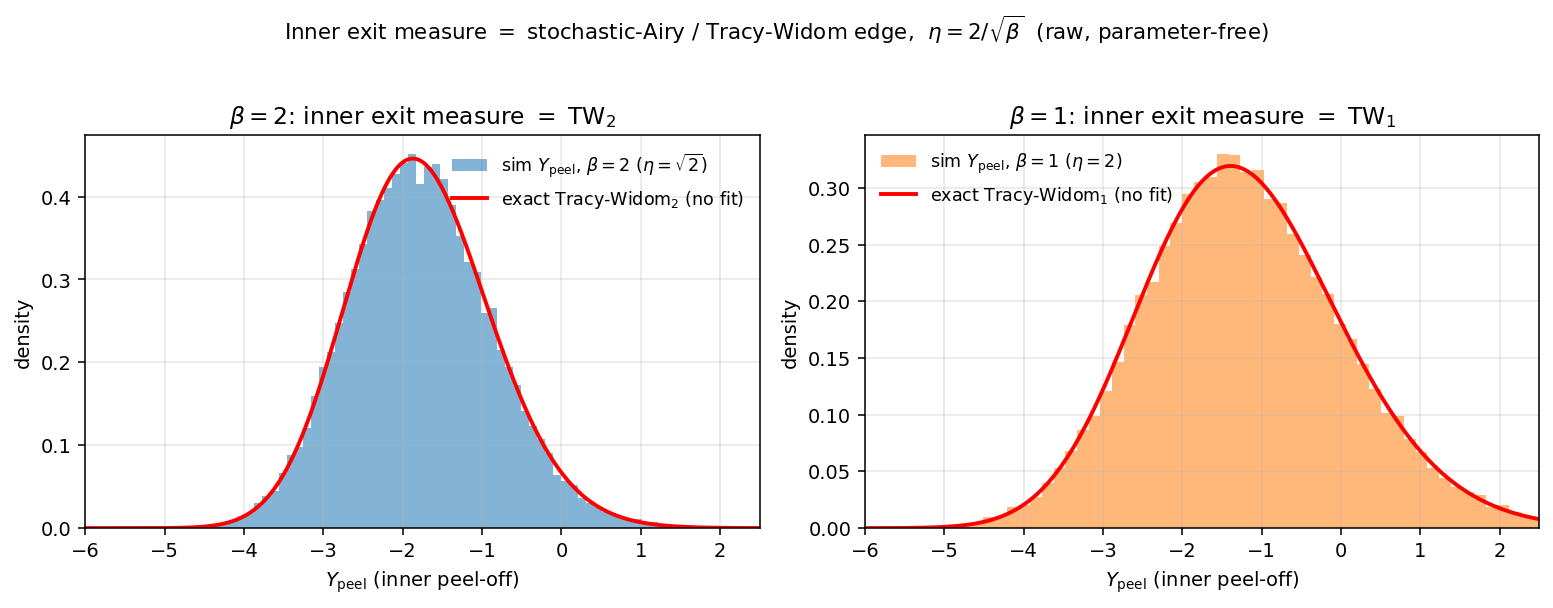
\includegraphics[width=0.92\textwidth]{figures/folded_cycle_tw_pdf.png}
\caption{The inner exit measure is Tracy--Widom, parameter-free. Raw Monte-Carlo histograms
of $\Ynode$ at $\beta=2$ ($\eta=\sqrt2$) and $\beta=1$ ($\eta=2$) overlaid on the exact
$\TW_2,\TW_1$ densities (Painlev\'e~II / Hastings--McLeod), with no centring, scaling or
fitting. Mean, variance, skewness and the asymmetric tail all match.}
\label{fig:twpdf}
\end{figure}

\begin{figure}[h]
\centering
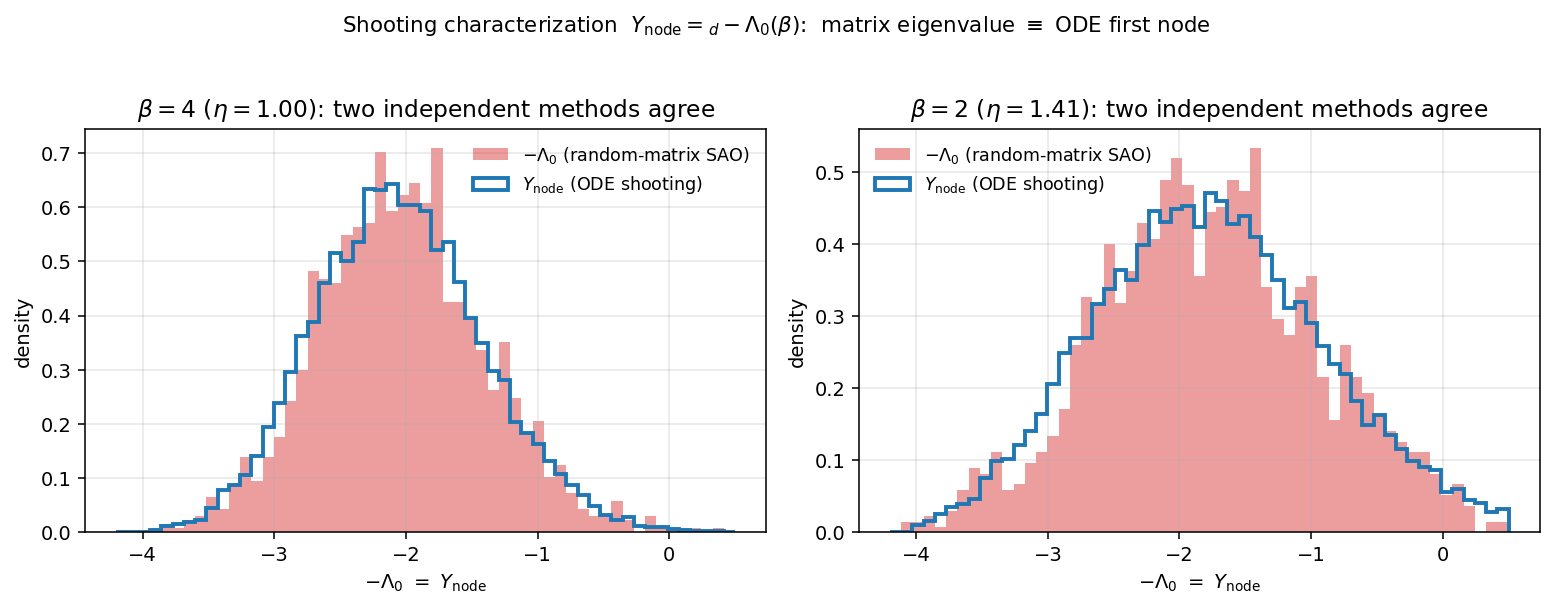
\includegraphics[width=0.92\textwidth]{figures/folded_cycle_shooting_duality.png}
\caption{Two independent methods agree. The peel-off law $\Ynode$ from ODE shooting (blue
step) and $-\Lam(\beta)$ from the smallest eigenvalue of a random-matrix discretisation of
$H_\beta$ (filled) coincide; the matrix computation knows nothing of sweeps or first nodes,
so the agreement is non-circular evidence for Theorem~\ref{thm:shoot}.}
\label{fig:dual}
\end{figure}

\begin{figure}[h]
\centering
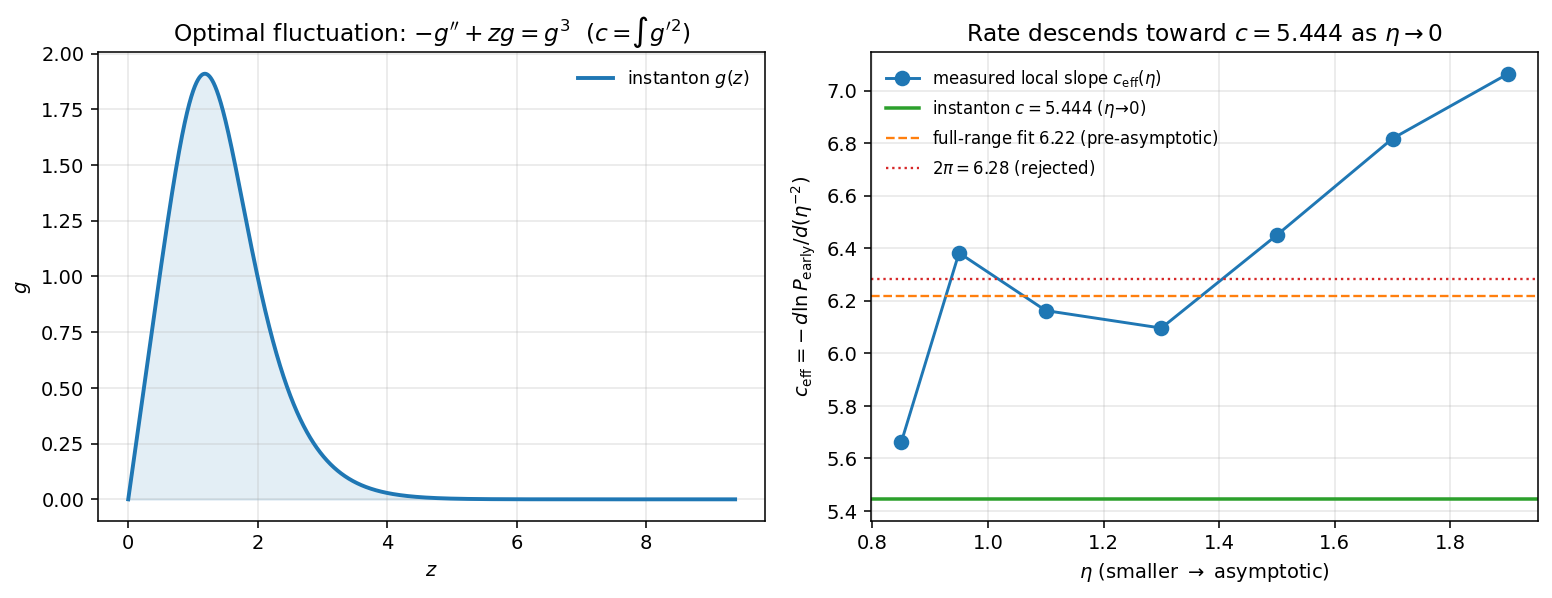
\includegraphics[width=0.92\textwidth]{figures/folded_cycle_rate_constant.png}
\caption{The rate constant. Left: the instanton (nonlinear-Airy ground state $-g''+xg=g^3$).
Right: the local slope $-\dd\log\Pearly/\dd(\eta^{-2})$ descends toward the Painlev\'e~II
value $c=5.444$ as $\eta\to0$; a single-window fit ($6.22$) and $2\pi$ are excluded.}
\label{fig:rate}
\end{figure}

Figure~\ref{fig:twpdf} shows the parameter-free Tracy--Widom overlay; the skewness tracks
$\TW_\beta$ along $\eta=2/\sqrt\beta$ with the dictionary as the only input. Figure
\ref{fig:dual} is the dual-method (ODE vs.\ random matrix) confirmation of
Theorem~\ref{thm:shoot}, agreeing in mean, variance and skewness at $\beta=1,2,4$. Figure
\ref{fig:rate} pins the rate constant $c=5.4439$ via the Painlev\'e~II instanton. The
early-escape tail $\Pearly=1-F_\beta(0)$ matches the exact Tracy--Widom CDF to Monte-Carlo
accuracy ($\beta=2$: $0.0298$ vs.\ $0.0306$; $\beta=1$: $0.1644$ vs.\ $0.1681$), and the
physical-variable simulation collapses in $\eta=\sigma/\sqrt{\ep_2}$ across a factor four in
$\ep_2$, confirming Proposition~\ref{prop:noise}. The phase exponent is measured at
$\omega\sim\sigma^{0.668}$, consistent with the proved $2/3$. Finally,
Figure~\ref{fig:breakdown} maps the regime of validity (Remark~\ref{rem:regime}): the
Tracy--Widom law is clean for $\eta\lesssim1$, while the recrossing that voids the
single-escape picture sets in beyond, along the Kramers boundary rather than at a fixed
$\eta$.

\begin{figure}[h]
\centering
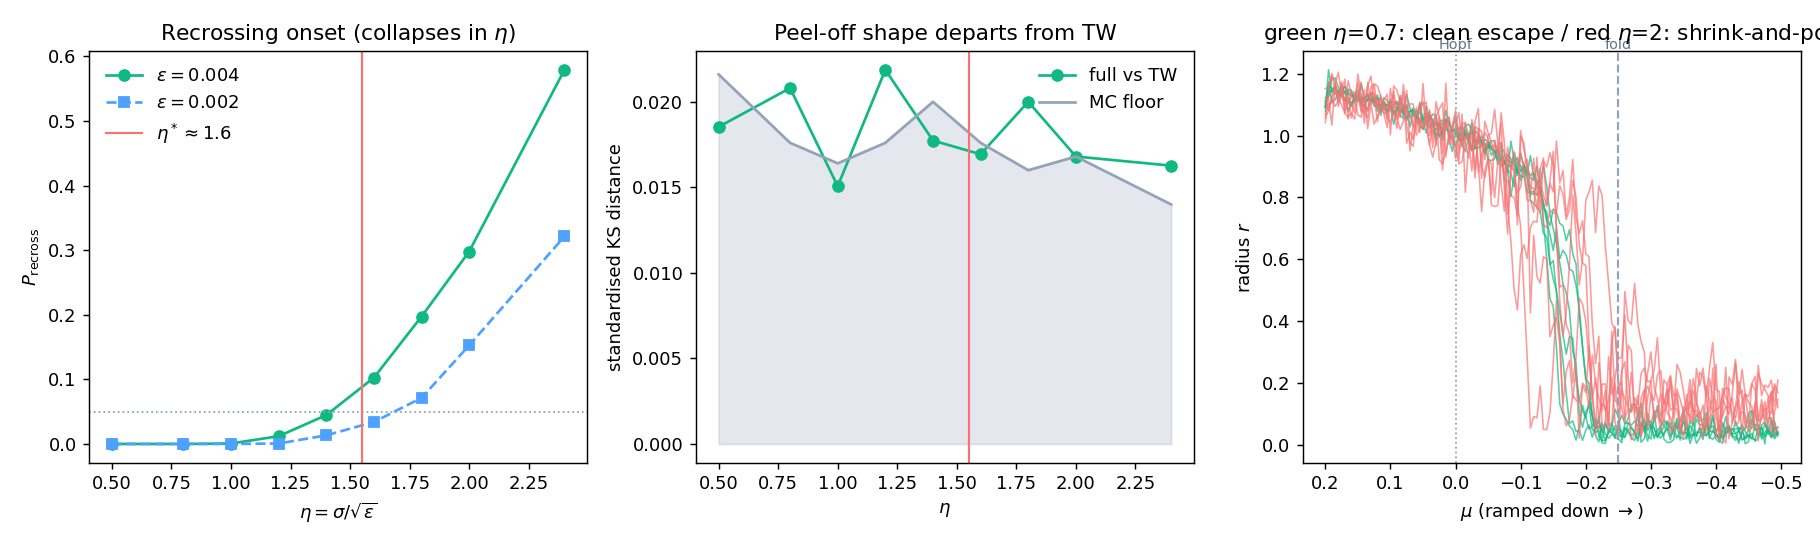
\includegraphics[width=0.98\textwidth]{figures/tw_breakdown.png}
\caption{Regime of validity of the Tracy--Widom law. \emph{Left:} recrossing probability
$P_{\rm recross}$ versus $\eta=\sigma/\sqrt{\ep_2}$ for two ramp rates---negligible for
$\eta\lesssim1$, rising through $5\%$ near $\eta\approx1.5$. The two rates do not collapse
because recrossing is a Kramers return ($\sim\ep_2^{-1}e^{-\Delta U/\sigma^2}$), not a function
of $\eta$ alone. \emph{Middle:} the standardised Kolmogorov--Smirnov distance between the
full-system peel-off and the canonical $\TW_\beta$ stays at the Monte-Carlo floor across the
range---the \emph{distribution} remains Tracy--Widom. \emph{Right:} sample radial trajectories;
one clean escape at the fold for $\eta=0.7$, shrink-and-pop recrossing for $\eta=2$.}
\label{fig:breakdown}
\end{figure}

\begin{figure}[h]
\centering
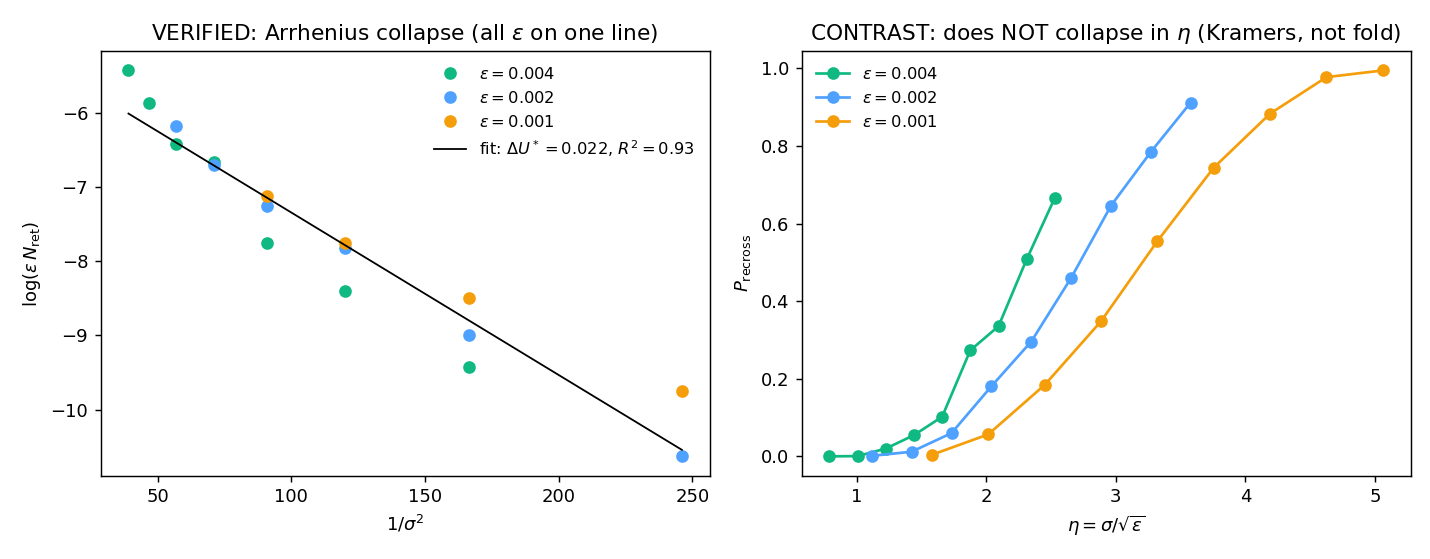
\includegraphics[width=0.92\textwidth]{figures/tw_boundary.png}
\caption{The recrossing boundary is Arrhenius, not a fixed $\eta$ (Remark~\ref{rem:regime}).
\emph{Left (verification):} $\log(\ep_2 N_{\rm ret})$ versus $1/\sigma^2$ for three ramp rates
collapses onto one line, $N_{\rm ret}=(C/\ep_2)e^{-\Delta U_*/\sigma^2}$ with
$\Delta U_*\approx0.022$ ($R^2=0.93$). \emph{Right (contrast):} the same data against
$\eta=\sigma/\sqrt{\ep_2}$ does \emph{not} collapse---the breakdown is a static-Kramers
$\sigma$-threshold (the classical $\sigma_{\rm crit}$), not the dynamic fold scale. The
Tracy--Widom regime $\sigma_*\sim\sqrt{\ep_2}$ sits below this ceiling.}
\label{fig:boundary}
\end{figure}

\section{Discussion}\label{sec:discussion}

\subsection{Universality}
The amplitude channel places the folded-cycle canard escape in the Tracy--Widom / KPZ edge
universality class. The mechanism is generic: any slow passage whose inner equation is the
Airy/Riccati canard, perturbed by white noise, Cole--Hopf-linearises to a Schr\"odinger
operator with white-noise potential, hence to the stochastic Airy operator. We therefore
expect the same $\TW_\beta$ exit law for noisy fold and folded-node passages, with $\beta$
read off the noise-to-curvature ratio $\eta=2/\sqrt\beta$. The two channels are the two
edges---an amplitude (Tracy--Widom) edge and a phase (saddle-node-on-circle) edge---and the
destroying bifurcation selects which is singular.

\subsection{Application}
Folded limit cycles organise the onset and offset of oscillation in slow--fast models of
excitable systems; the inner exit measure is the law of the slow variable at the moment the
oscillation is lost, i.e.\ the timing statistics of noise-induced transitions. The
prediction is concrete: in the small-noise regime $\eta\lesssim1$ (Remark~\ref{rem:regime})
those statistics are Tracy--Widom, with the noise-induced jump scales
$(r,y)\sim(\sigma^{2/3},\sigma^{4/3})$ and critical noise $\sigma_*\sim\sqrt{\ep_2}$; for
larger noise the coexisting rest state renders the transition two-way and rate-governed.

\subsection{Early warning of bifurcations}
The dichotomy has an operational reading. Approached adiabatically, a folded cycle announces
its destroying bifurcation through whichever channel is singular. At a phase edge (saddle-node
on the invariant circle, or saddle-homoclinic) the inter-event period diverges and the
dimensionless timing statistics---the coefficient of variation and the rescaled
first-passage shape---collapse onto the universal law, so the rescaled distance to threshold
is identifiable from the event timing alone and its approach to zero is the precursor; at an
amplitude edge (Hopf, or fold of cycles) the period stays finite and the timing is blind,
while the oscillation amplitude is the singular observable. We have checked this numerically
across the four canonical onset/offset bifurcations: drifting the parameter slowly through
each, the timing precursor fires precisely at the phase edges and is silent at the amplitude
edges, where the amplitude collapses instead. The supercritical Hopf collapse is gradual---an
amplitude precursor---whereas the fold of cycles holds its amplitude and then jumps, leaving
no precursor in either channel; the edge classification thus also identifies the bifurcations
against which time-series early warning is intrinsically powerless. Two caveats temper the
prescription. It is adiabatic: the system must dwell near threshold long enough for the
universal inner law to form, so a fast, slow-variable--driven offset (as in the Epileptor)
terminates the oscillation before the period diverges and carries no timing precursor. And the
universal timing shape is the near-threshold, noise-dominated one; a relaxation oscillator's
regular firing departs from it away from threshold. Within these limits the two-edge structure
furnishes a bifurcation-specific early-warning signal---calibrated and confound-robust where
generic critical-slowing-down statistics are not---selected by the destroying bifurcation.

\subsection{Open problems}
The constant $c=5.4439$ is a definite Painlev\'e~II action whose elementary closed form, if
any, is open. The phase-channel constant $J$ has slowly-converging tails and its universal
first-passage law lacks a Tracy--Widom-style closed form. A fully self-contained treatment
would internalise the RRV operator construction and the Berglund--Gentz tubes rather than
cite them. Finally, the Tracy--Widom identification suggests finer KPZ-class objects (the
Airy process) may govern the joint law of successive peel-offs in a forced or coupled
folded cycle.

\subsection*{Acknowledgements}
The author thanks N.\ Popovi\'c for supervision and the JKK deterministic backbone.

\begin{thebibliography}{9}
\bibitem{KS} M.~Krupa, P.~Szmolyan, \emph{Extending geometric singular perturbation theory
to nonhyperbolic points---fold and canard points in two dimensions}, SIAM J.\ Math.\ Anal.\
\textbf{33} (2001) 286--314.
\bibitem{JKK} S.~Jelbart, C.~Kuehn, N.~Kuntz, \emph{Geometric blow-up of a dynamic
Hopf/fold-of-cycles}, arXiv:2208.01361 (2024).
\bibitem{RRV} J.~A.~Ram\'irez, B.~Rider, B.~Vir\'ag, \emph{Beta ensembles, stochastic Airy
spectrum, and a diffusion}, J.\ Amer.\ Math.\ Soc.\ \textbf{24} (2011) 919--944.
\bibitem{BG} N.~Berglund, B.~Gentz, \emph{Noise-Induced Phenomena in Slow--Fast Dynamical
Systems: A Sample-Paths Approach}, Springer, 2006.
\bibitem{BGK} N.~Berglund, B.~Gentz, C.~Kuehn, \emph{Hunting French ducks in a noisy
environment}, J.\ Differential Equations \textbf{252} (2012) 4786--4841; \emph{From random
Poincar\'e maps to stochastic mixed-mode-oscillation patterns}, J.\ Dynam.\ Differential
Equations \textbf{27} (2015) 83--136.
\bibitem{TW} C.~A.~Tracy, H.~Widom, \emph{Level-spacing distributions and the Airy kernel},
Comm.\ Math.\ Phys.\ \textbf{159} (1994) 151--174.
\bibitem{Bornemann} F.~Bornemann, \emph{On the numerical evaluation of distributions in
random matrix theory: a review}, Markov Process.\ Related Fields \textbf{16} (2010)
803--866.
\bibitem{DZ} A.~Dembo, O.~Zeitouni, \emph{Large Deviations Techniques and Applications},
2nd ed., Springer, 1998.
\bibitem{Reimann} P.~Reimann et al., \emph{Giant acceleration of free diffusion by use of
tilted periodic potentials}, Phys.\ Rev.\ Lett.\ \textbf{87} (2001) 010602.
\bibitem{Corwin} I.~Corwin, \emph{The Kardar--Parisi--Zhang equation and universality
class}, Random Matrices Theory Appl.\ \textbf{1} (2012) 1130001.
\bibitem{ET} G.~B.~Ermentrout, D.~Terman, \emph{Mathematical Foundations of Neuroscience},
Springer, 2010.
\end{thebibliography}

\end{document}
